\section{Geometric ergodicity}

\subsection{Synthetic MJP}

  \begin{figure}[H]
  \centering
  \begin{minipage}[hp]{0.45\linewidth}
  \centering
    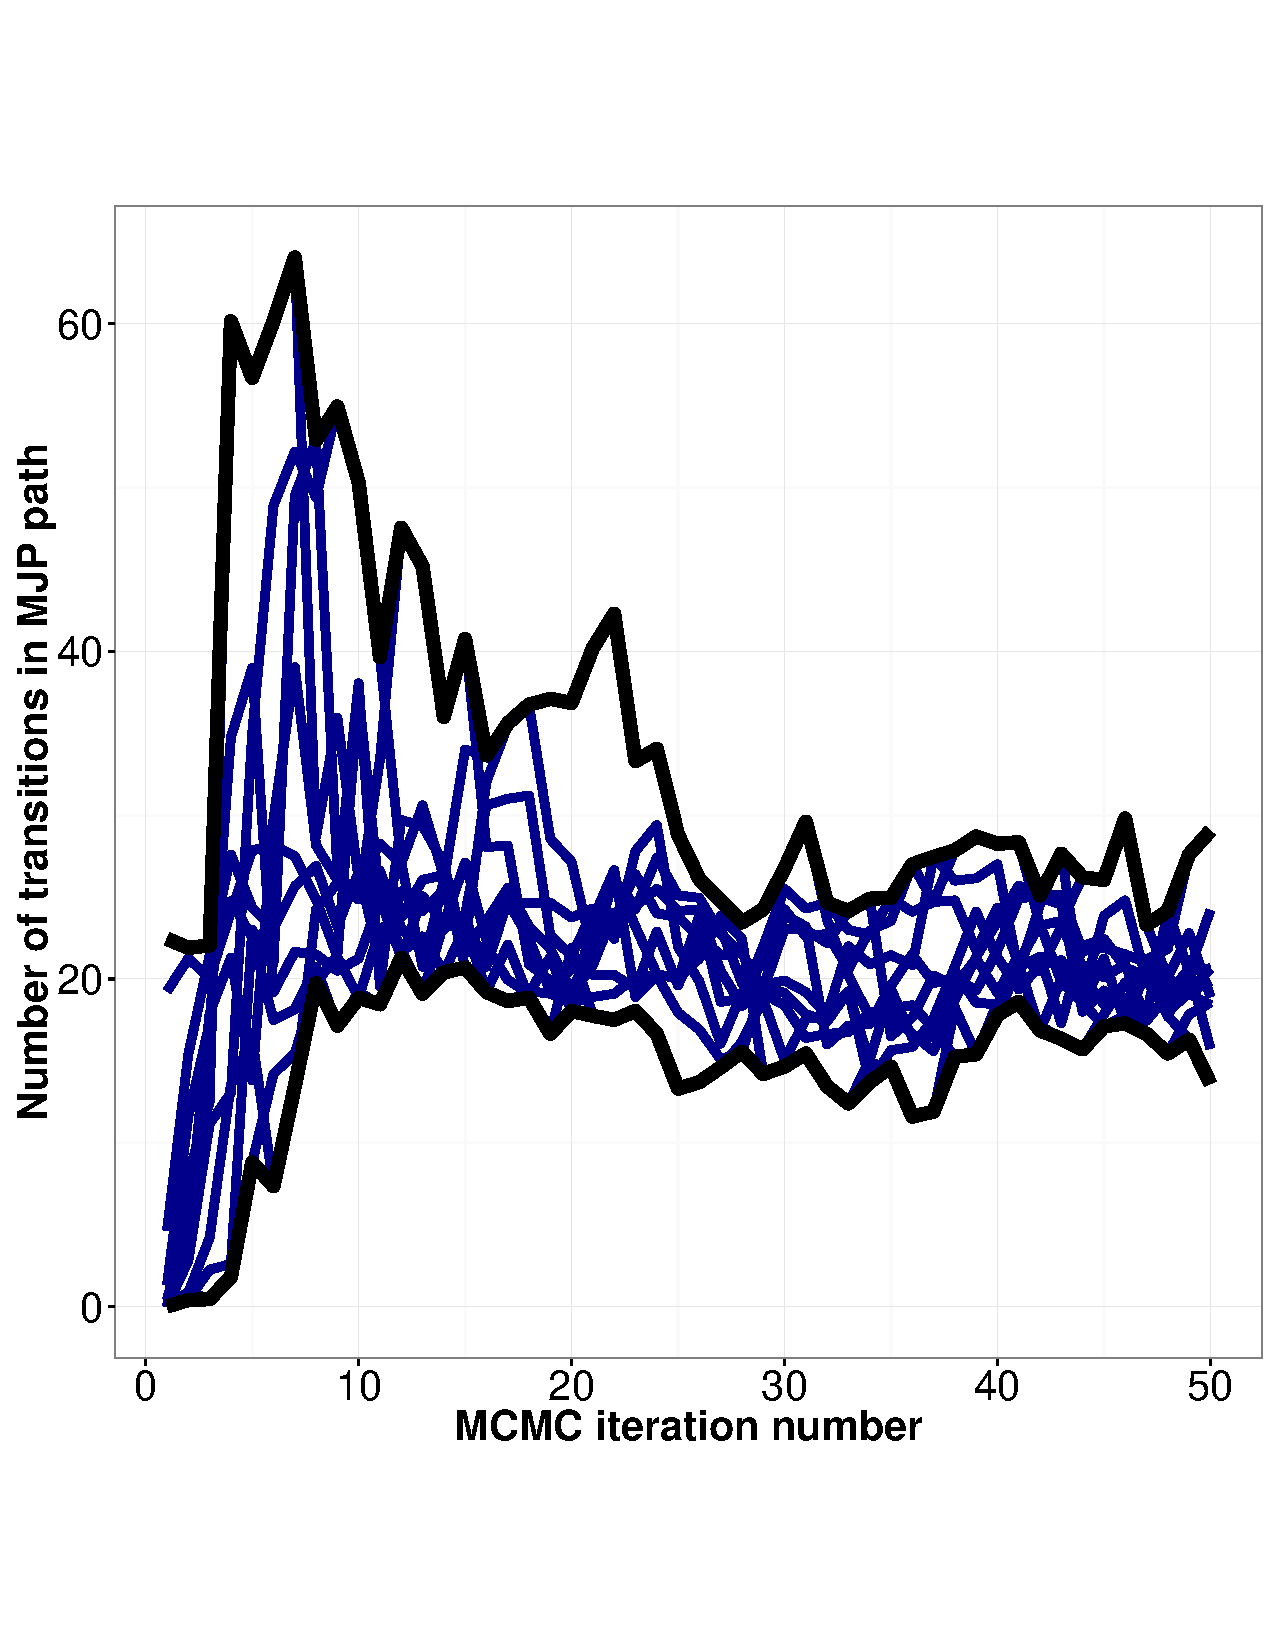
\includegraphics [width=0.90\textwidth, angle=0]{figs/exp3_k2_path_transition.pdf}
      \end{minipage}
    \caption{Trace plot of the number of MJP transitions for different initializatoins.}
	\label{fig:Transition_exp}
  \end{figure}

Figure~\ref{fig:Transition_exp} shows the initial burn-in of our improved MH 
sampler for the immigration-death model for different initializations. The vertical 
axis shows the number of state transitions in the MJP trajectory of each iteration. 
This quantity quickly reaches its equilibrium value within a few iterations.\\

% \begin{figure}[H]
% \centering
% \begin{minipage}[hp]{0.45\linewidth}
% \centering
%   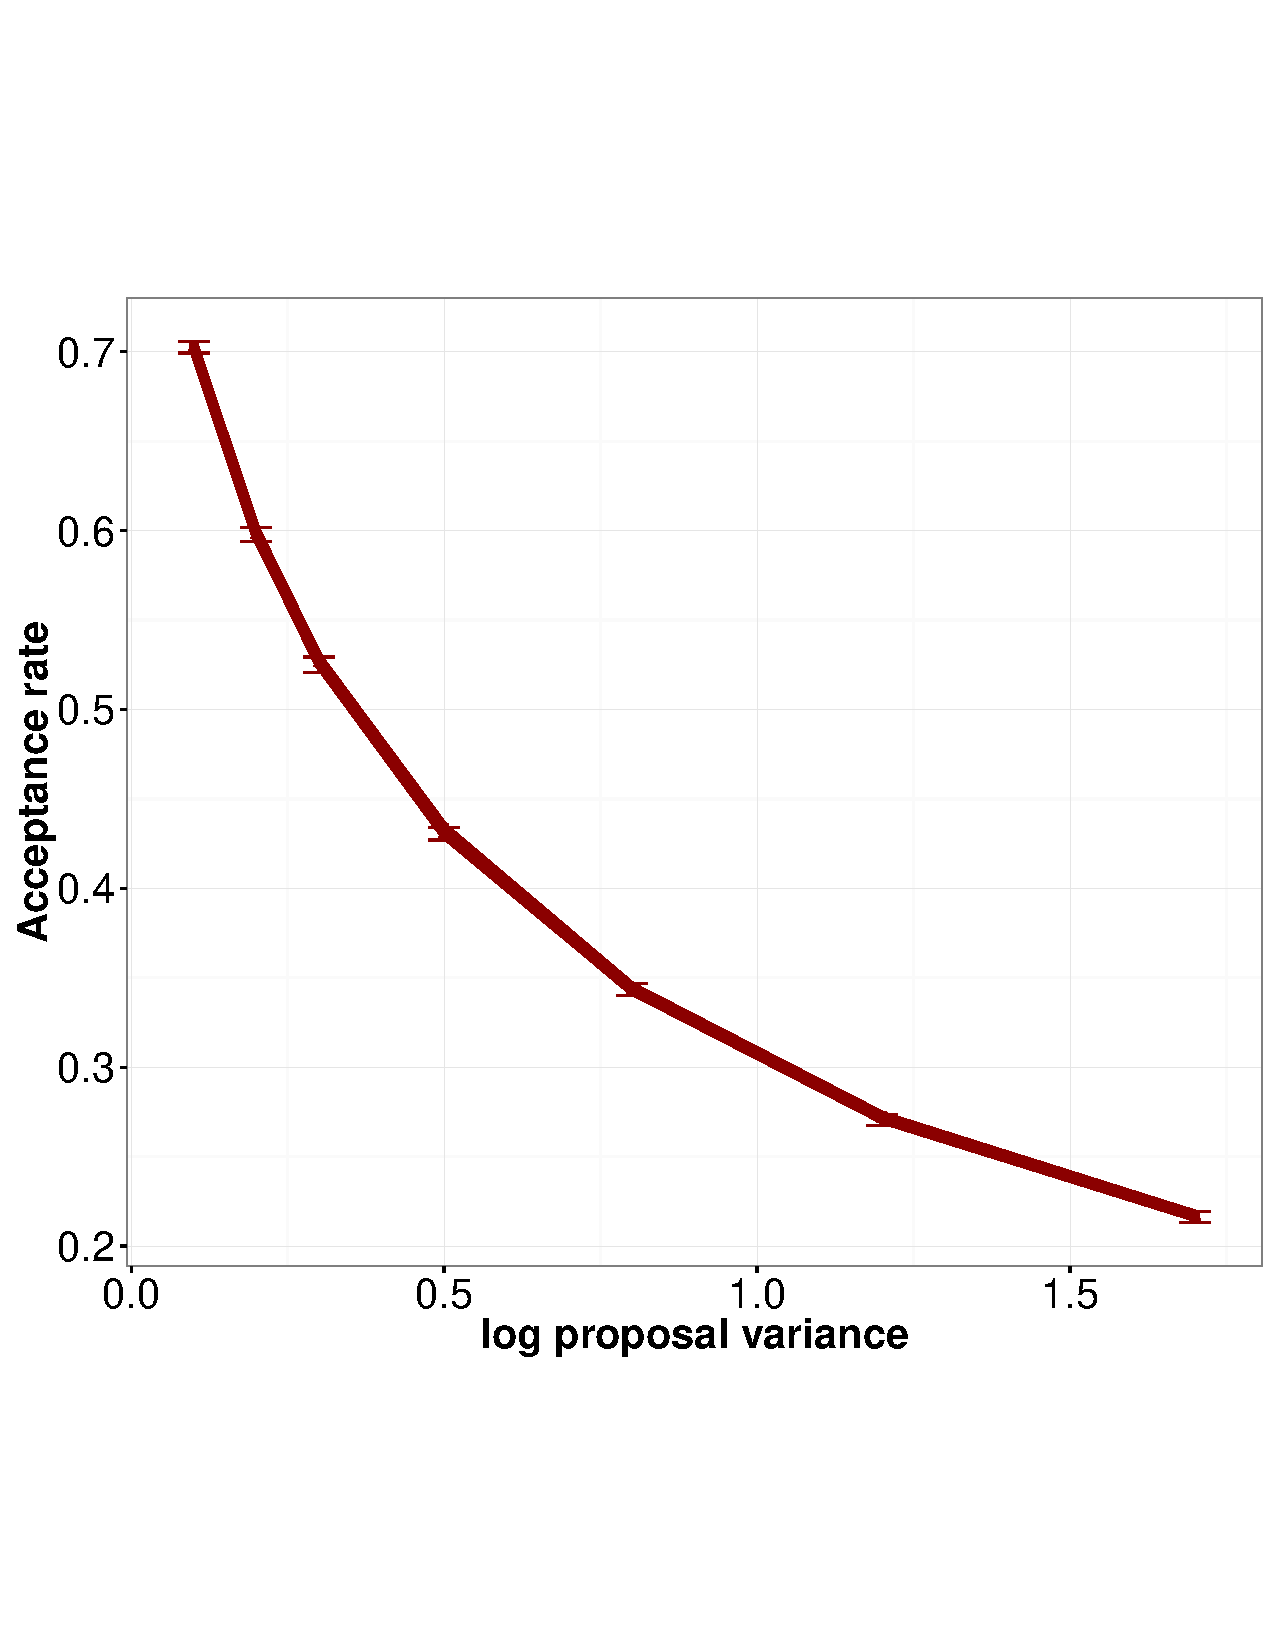
\includegraphics [width=0.90\textwidth, angle=0]{figs/acc_rate_exp_d3.pdf}
%     \end{minipage}
%   \caption{Acceptance rate for exp model (dim 3)}
%   \label{fig:acc_exp}
% \end{figure}

% Figure~\ref{fig:acc_exp} plots ESS plots the overall  acceptance rate against 
% the log variance of the proposal kernel per run for dimension $3$. 



  
    \begin{figure}[H]
  \centering
  \begin{minipage}[hp]{0.45\linewidth}
  \centering
    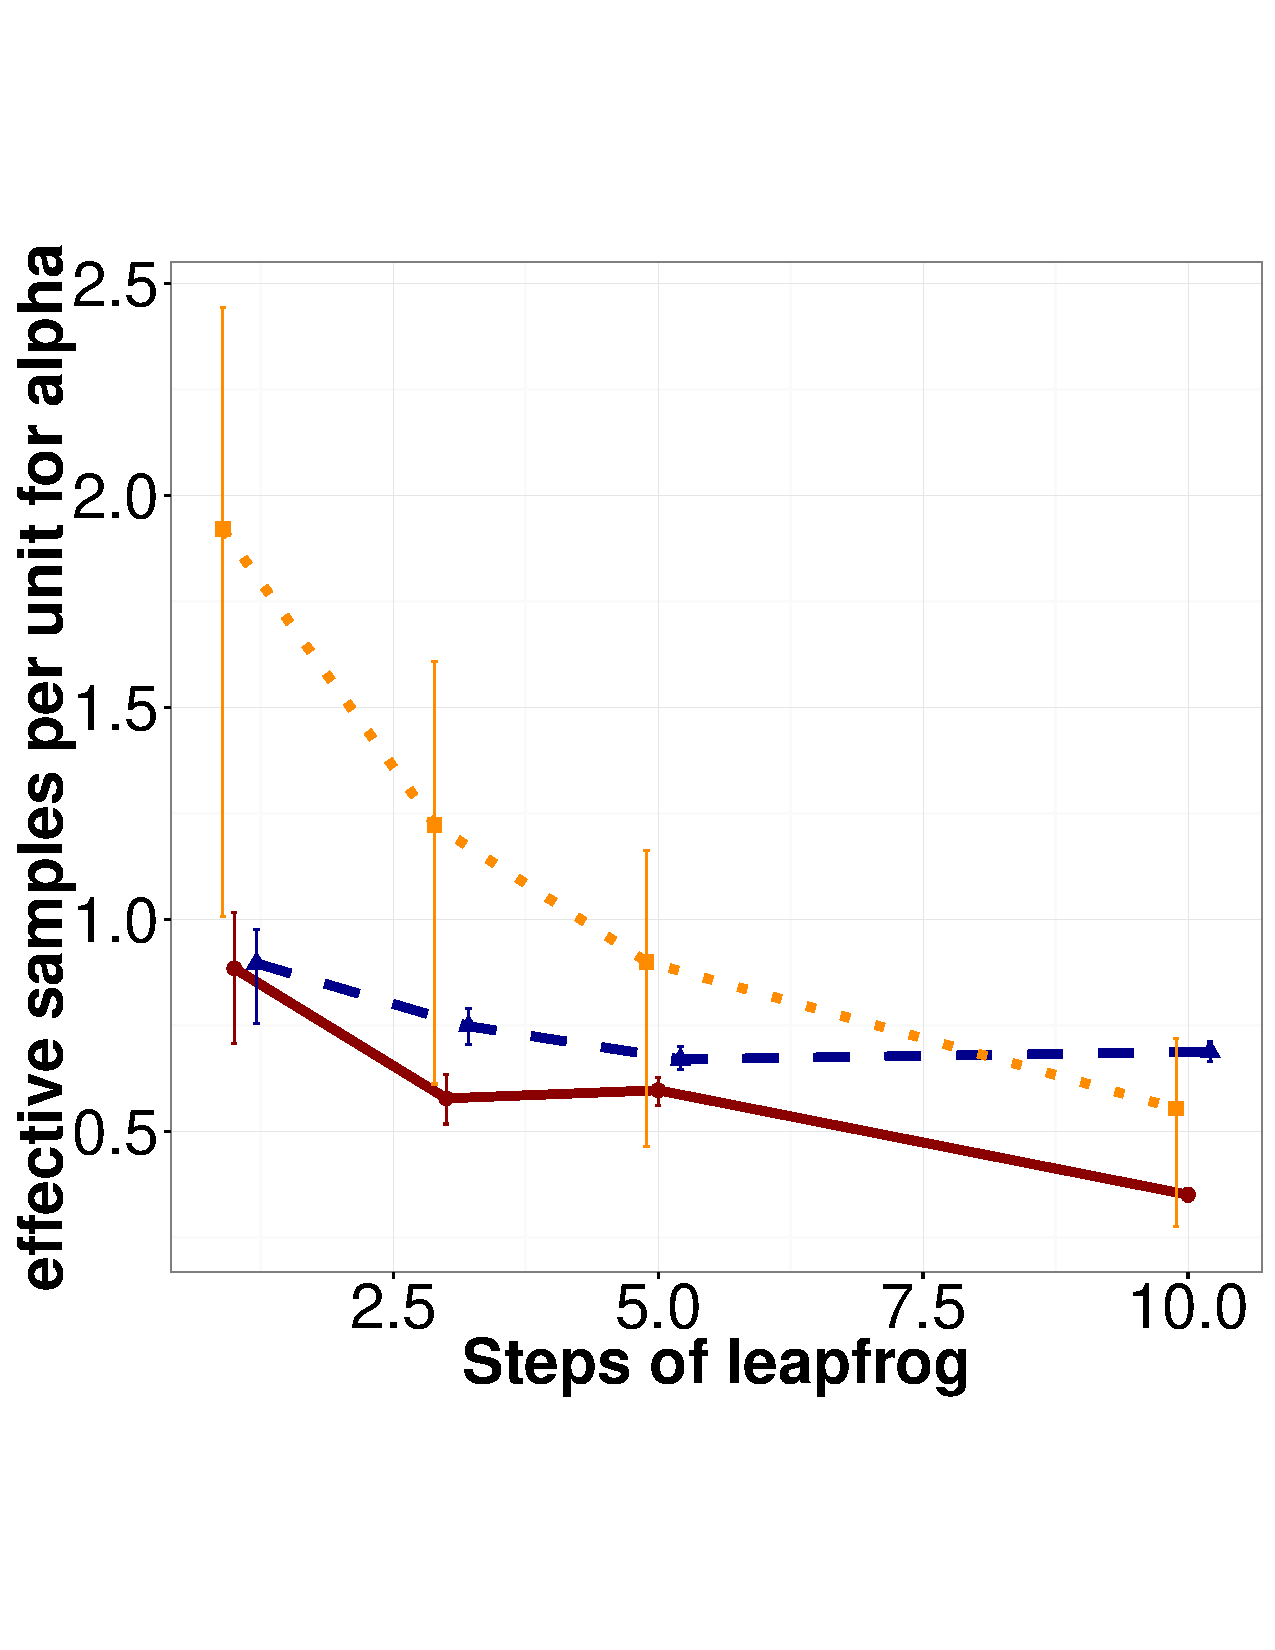
\includegraphics [width=0.90\textwidth, angle=0]{figs/h_alpha.pdf}
      \end{minipage}
  \begin{minipage}[hp]{0.45\linewidth}
  \centering
    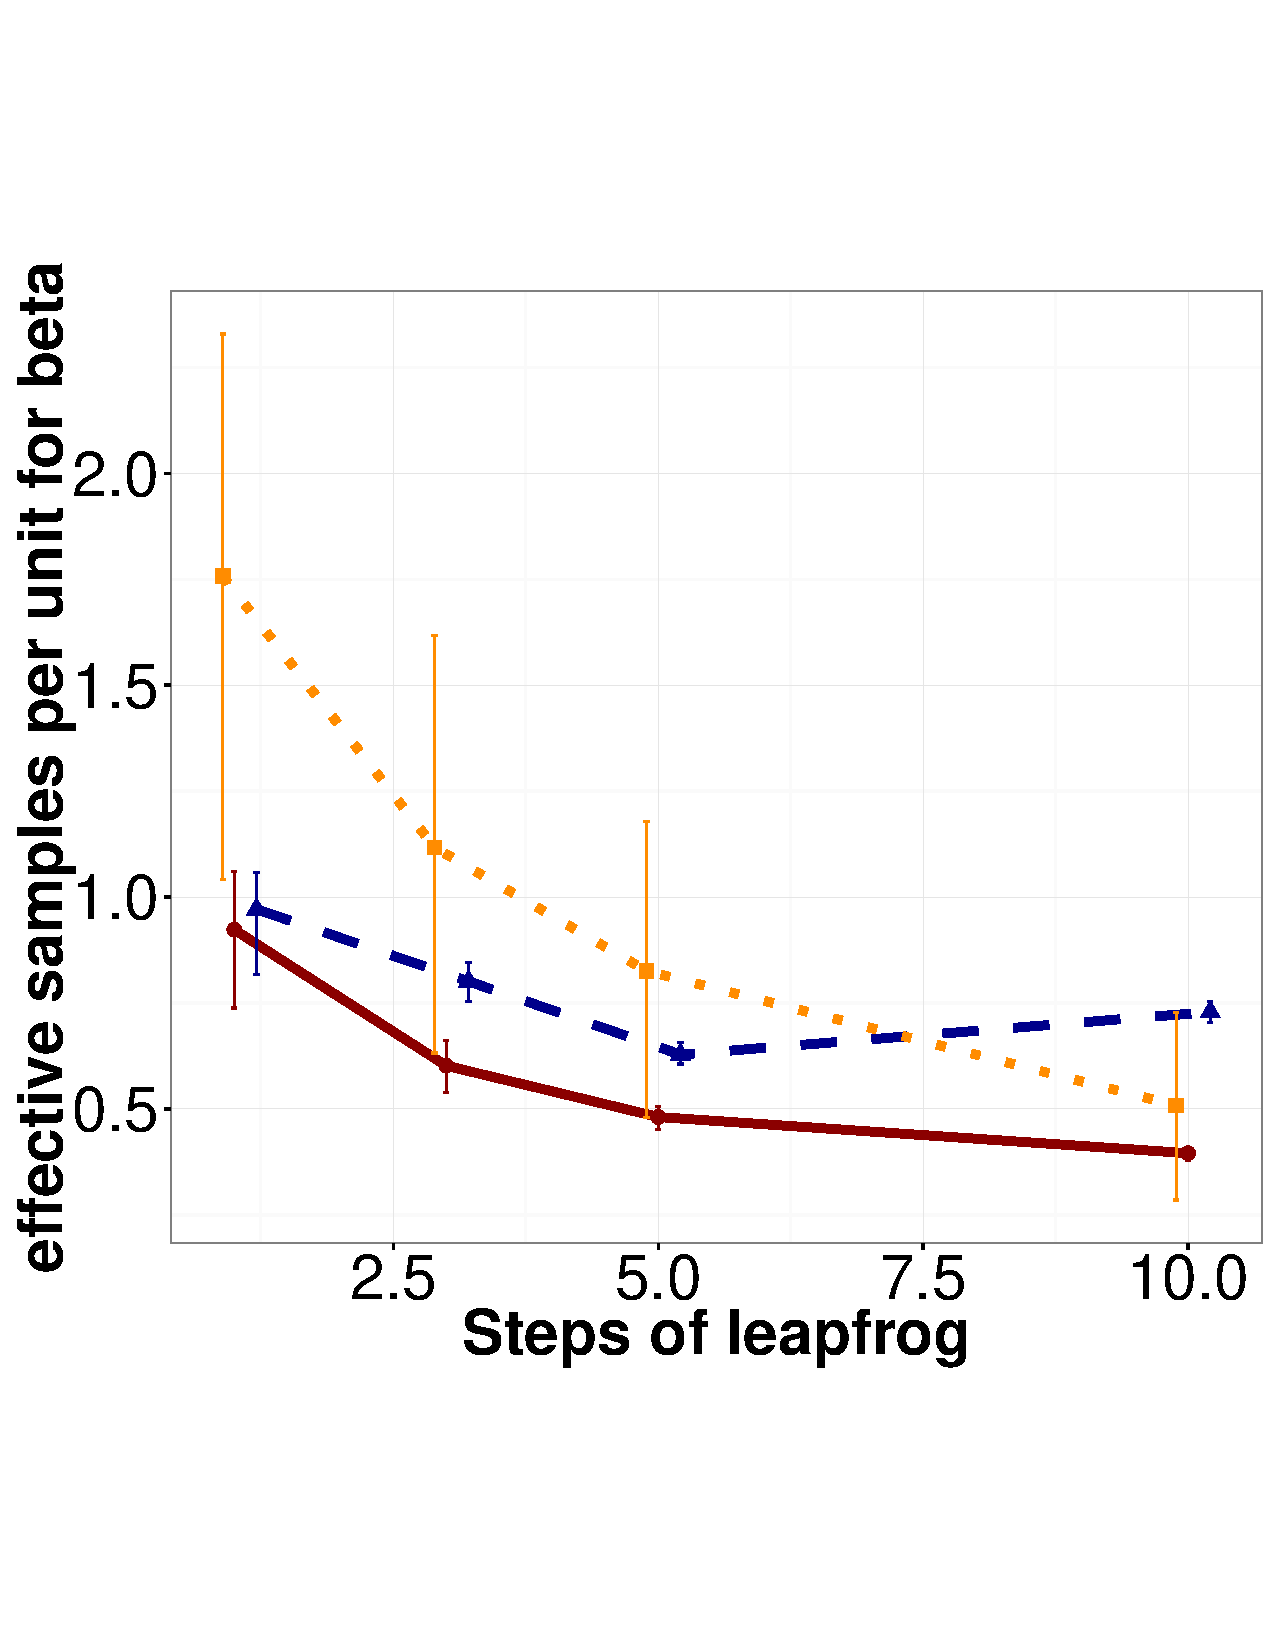
\includegraphics [width=0.90\textwidth, angle=0]{figs/h_beta.pdf}
      \end{minipage}
    \caption{HMC for dim 3}
    \label{fig:HMC_DIM_3}
  \end{figure}
In Figure~\ref{fig:HMC_DIM_3}, we plot the ESS per unit time as we change the 
number of leapfrog jumps in Hamiltonian MCMC for dimension $3$ for the 
immigration-death model. We consider 
three different step size for leapfrog step($s = 0.02, 0.05, 0.1$). 
% We use the same data for our previous experiment for the case when dimension $3$. 
We set the mass matrix $M$ to the identity matrix. We see that in this case,
the improved exploration afforded by HMC is not sufficient to overcome the 
computational burden it incurs: this is partly because every time a gradient is
computed (and this every leapfrog step), one needs to run the forward-backward algorithm.

  \begin{figure}[H]
  \centering
  \begin{minipage}[!hp]{0.45\linewidth}
  \centering
    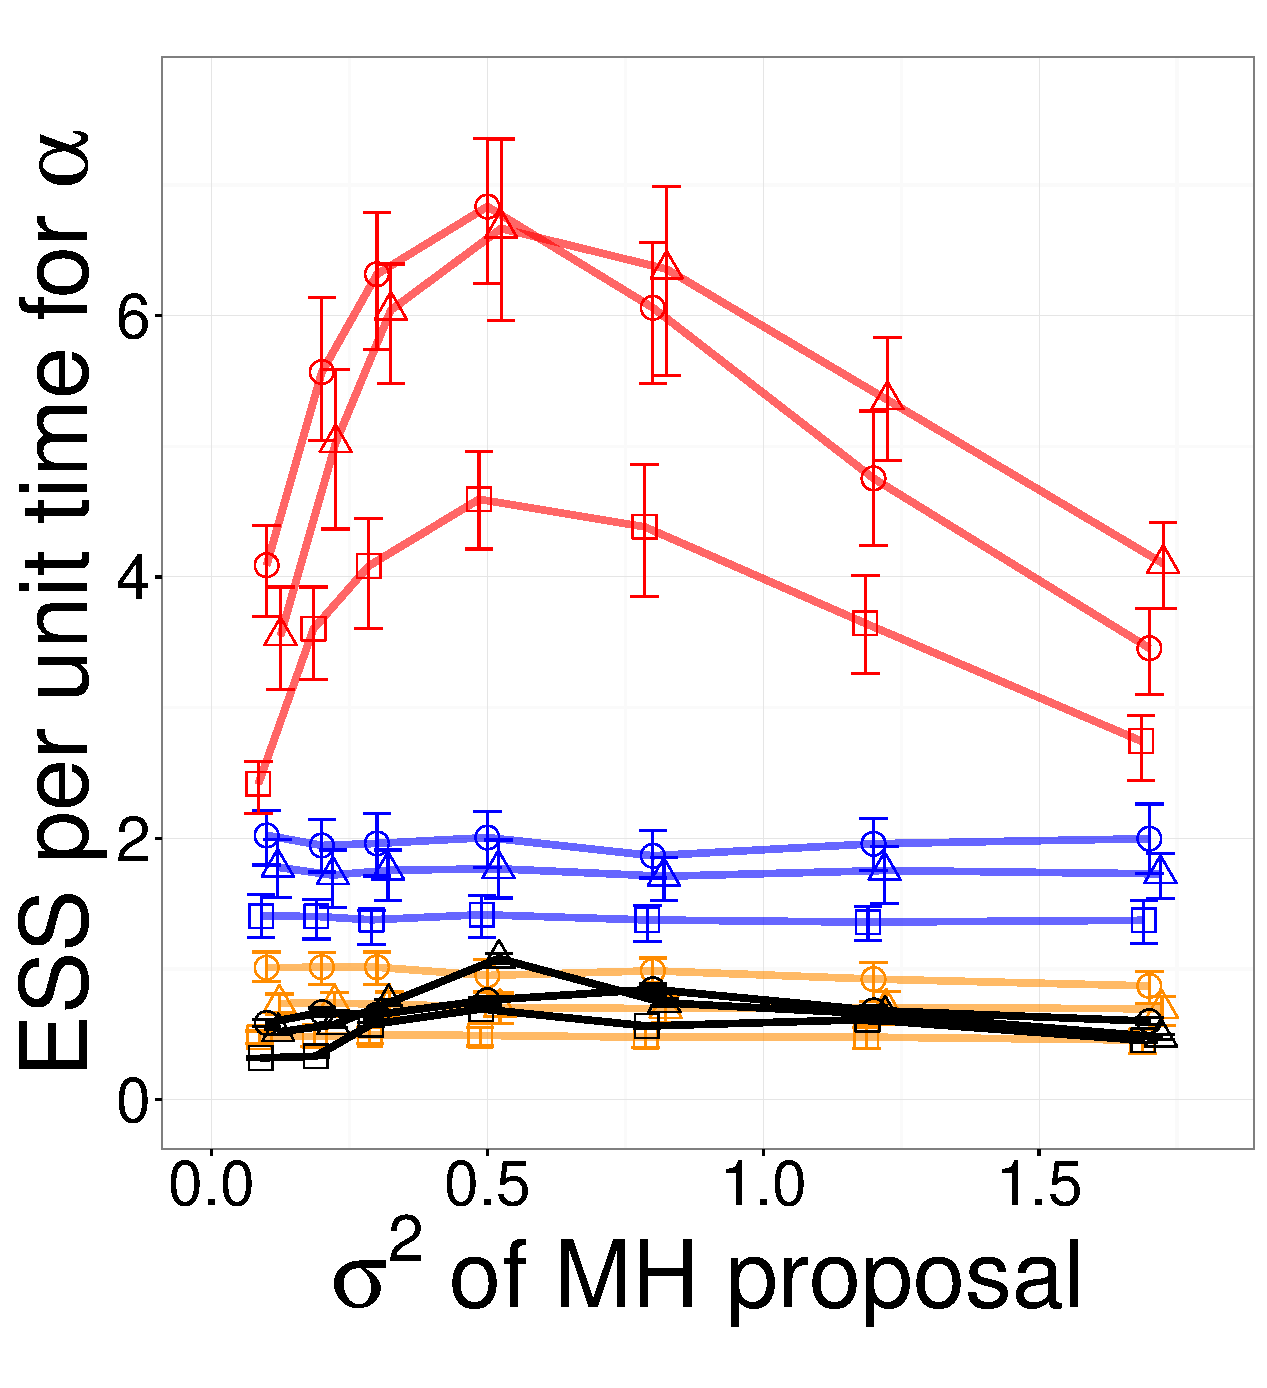
\includegraphics [width=0.90\textwidth, angle=0]{figs/exp_5_alpha.pdf}
      \end{minipage}
  \begin{minipage}[hp]{0.45\linewidth}
  \centering
    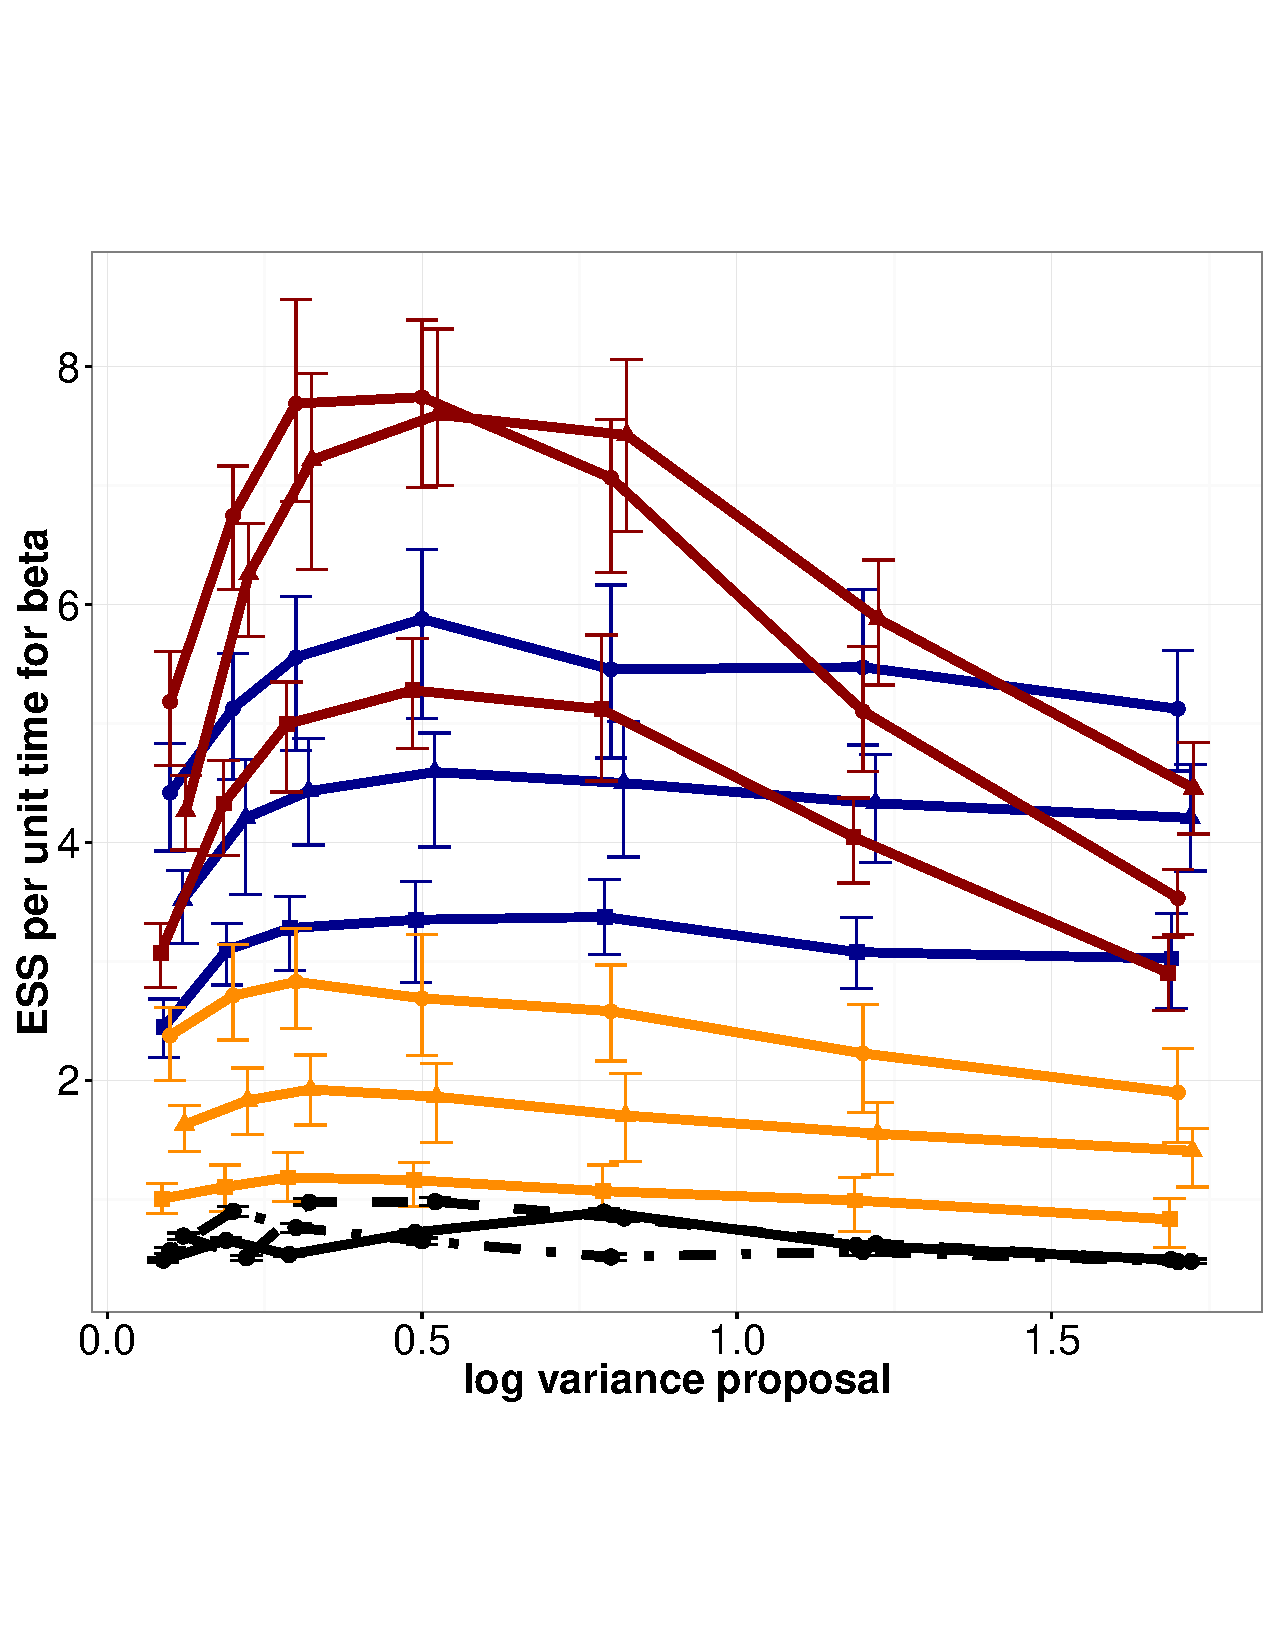
\includegraphics [width=0.90\textwidth, angle=0]{figs/exp_5_beta.pdf}
    \vspace{-0 in}
  \end{minipage}
    \caption{ESS/sec for the synthetic model with dimension 5. The left is for 
    $\alpha$, and the right is for $\beta$.}
     \label{fig:ESS_EXP_D5}
  \end{figure}

\subsection{Immigration model with capacity}
\begin{figure}[H]
  \begin{minipage}[hp]{0.85\linewidth}
  \centering
    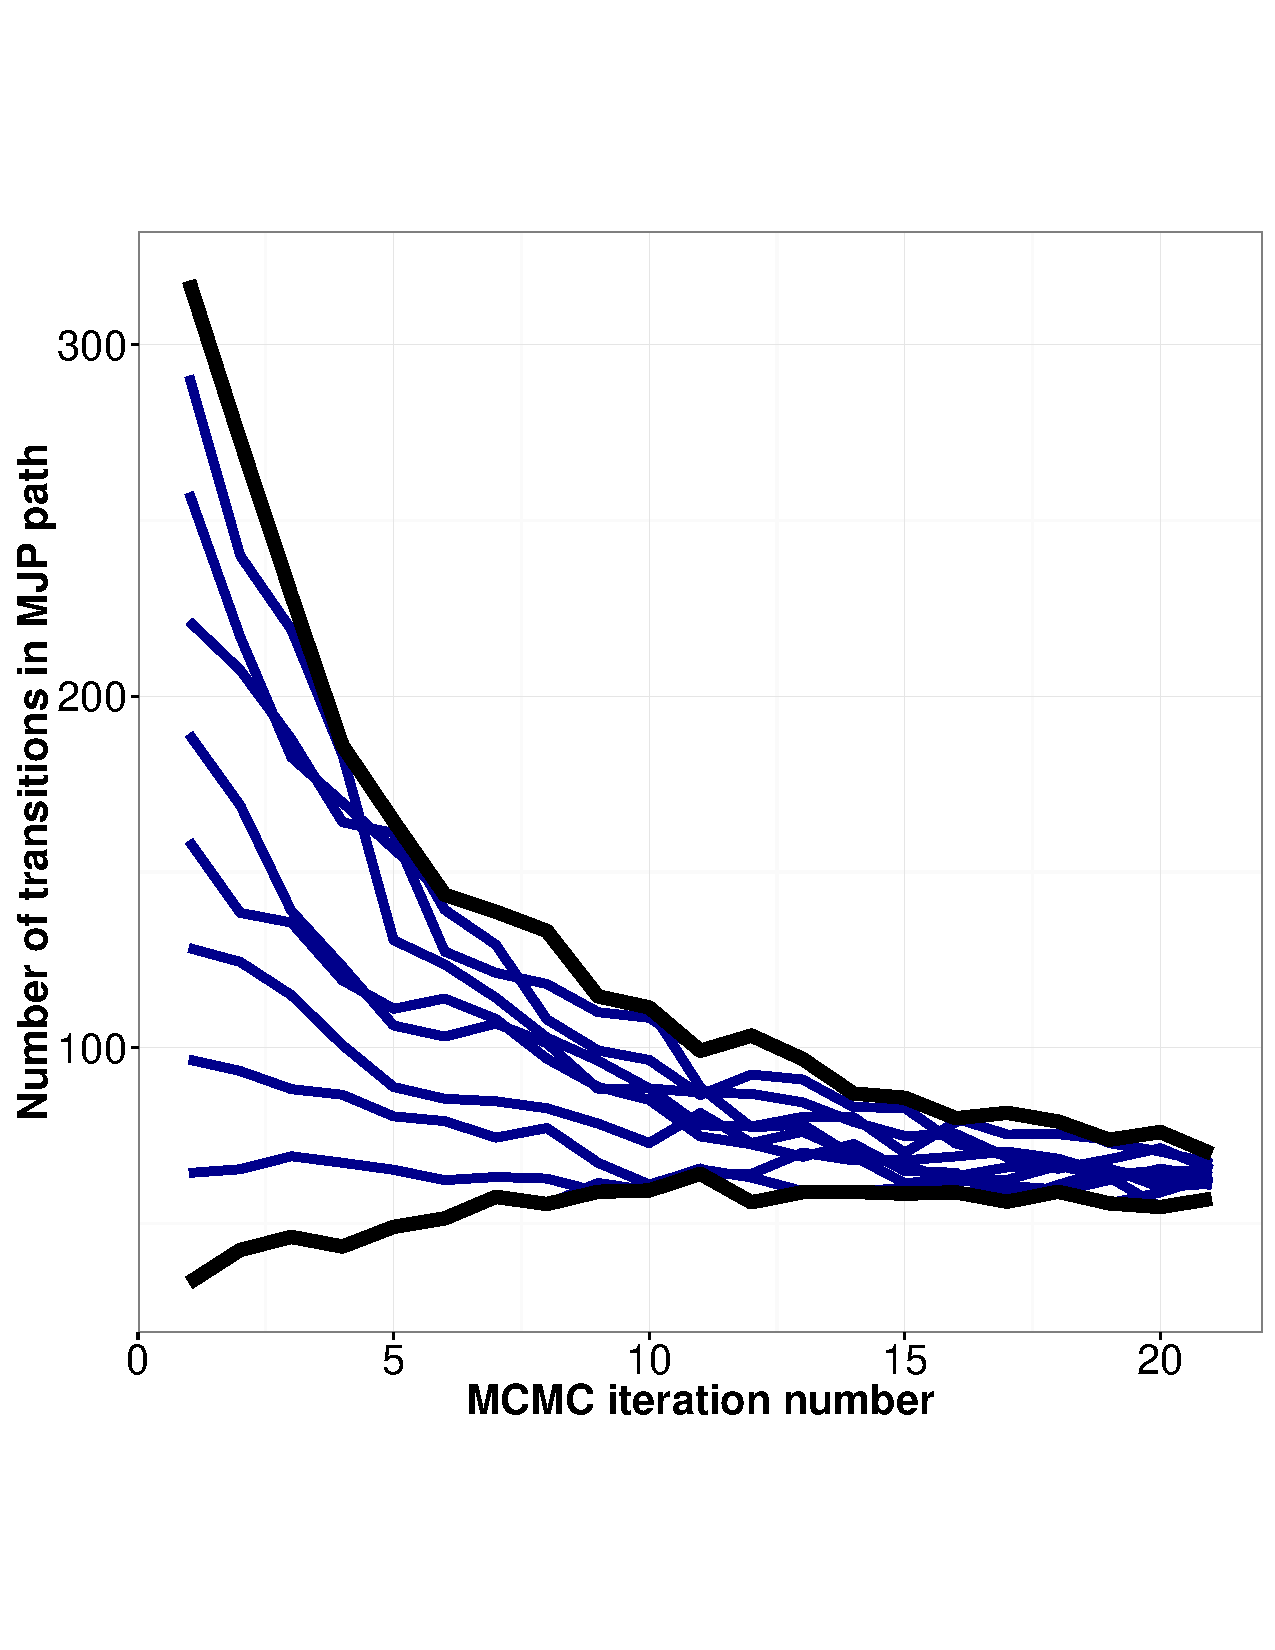
\includegraphics [width=0.40\textwidth, angle=0]{figs/q3_k2_path_transition.pdf}
    \vspace{-0 in}
    \caption{Trace plot of the number of MJP transitions for different initializatoins for immigration model.}
     \label{fig:ESS_Q_TRANSITION}
  \end{minipage}
\end{figure}

  \begin{figure}[H]
  \centering
  \begin{minipage}[hp]{0.45\linewidth}
  \centering
    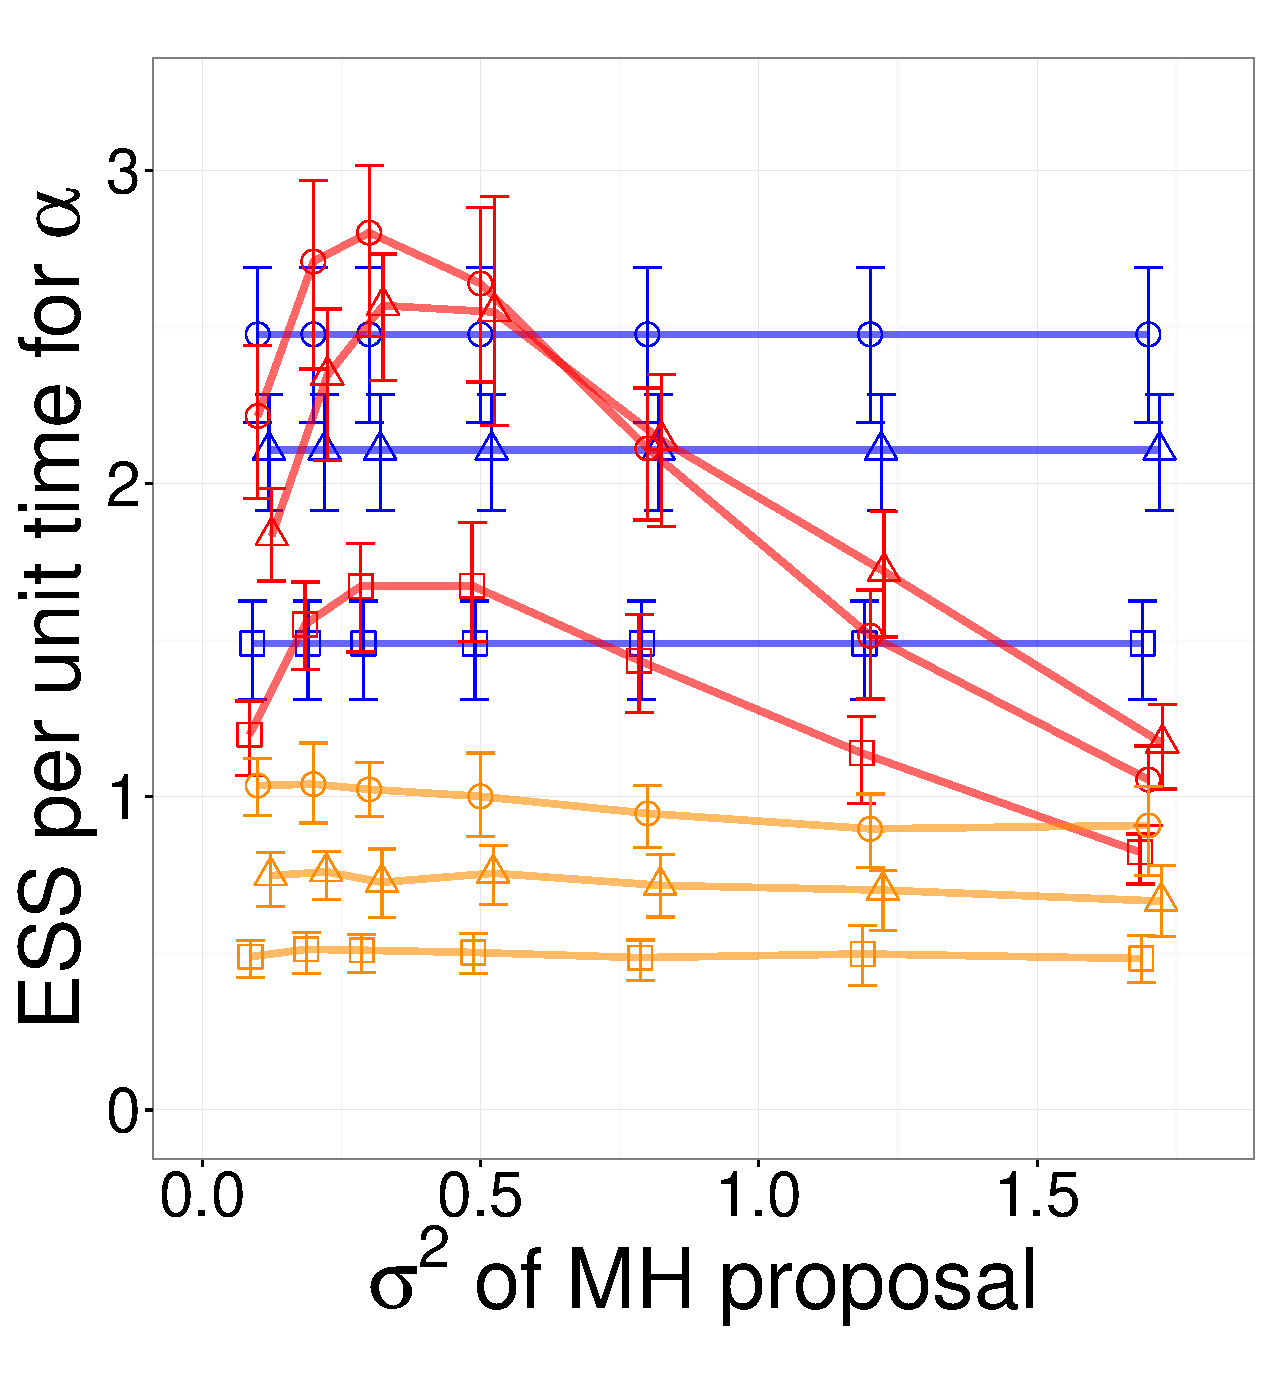
\includegraphics [width=0.90\textwidth, angle=0]{figs/q_5_alpha.pdf}
      \end{minipage}
  \begin{minipage}[hp]{0.45\linewidth}
  \centering
    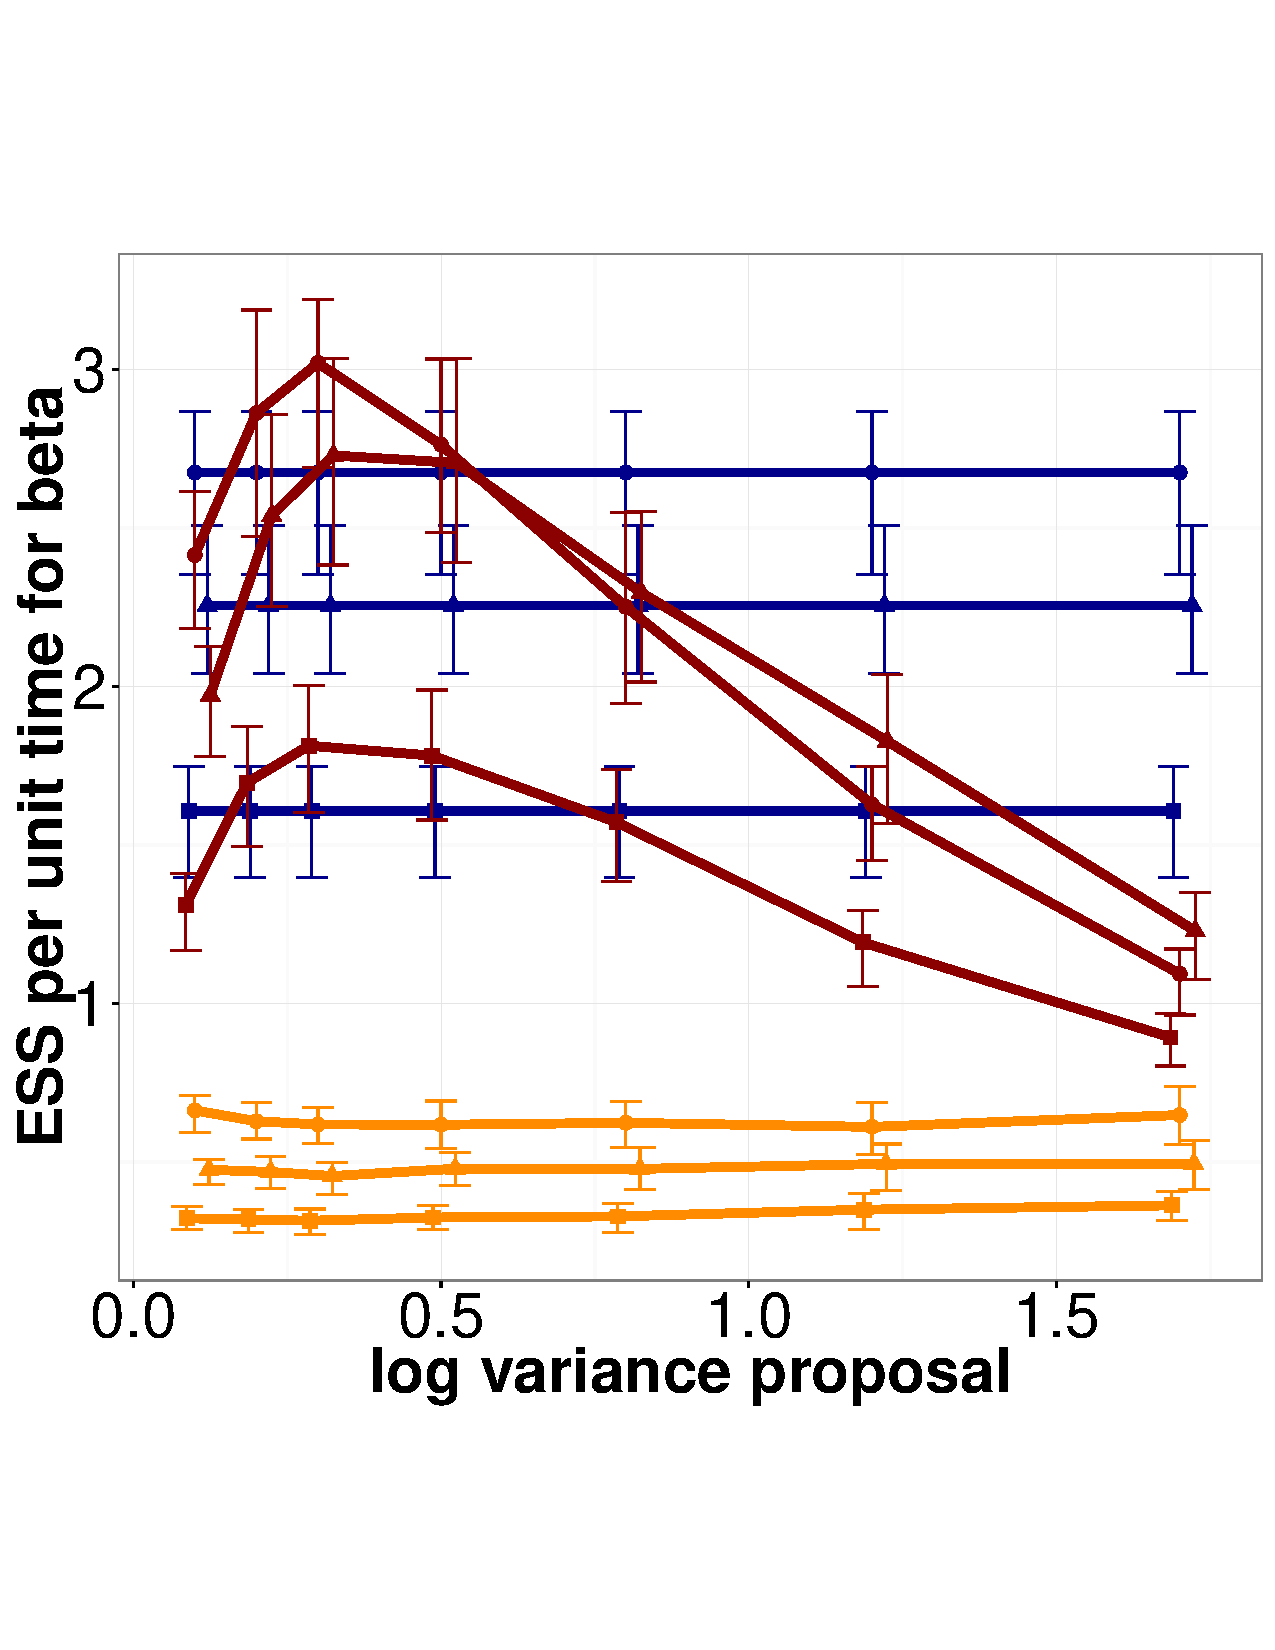
\includegraphics [width=0.90\textwidth, angle=0]{figs/q_5_beta.pdf}
    \vspace{-0 in}
      \label{fig:ESS_Q_D5}
  \end{minipage}
    \caption{ESS/sec for Immigration model (dim 5).The left is for $\alpha$, and the right is for $\beta$.}
  \end{figure}

\subsection{Non-homogeneous immigration model}

  \begin{figure}[H]
  \centering
  \begin{minipage}[!hp]{0.45\linewidth}
  \centering
    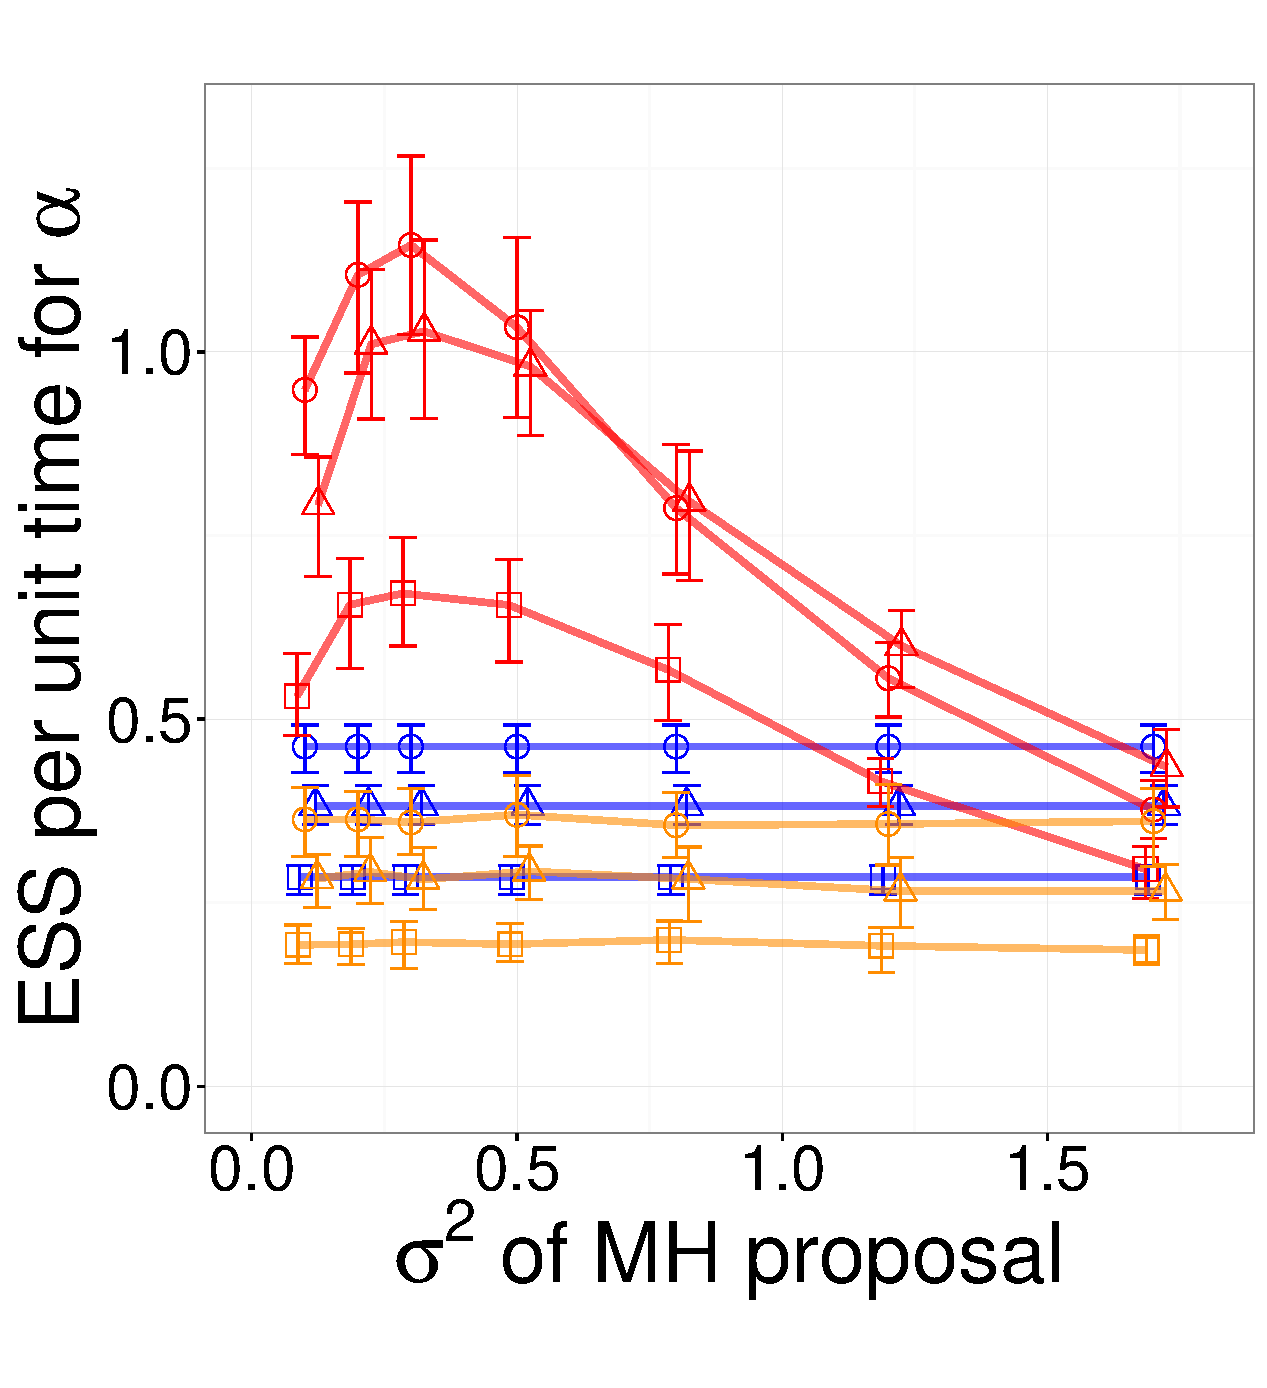
\includegraphics [width=0.950\textwidth, angle=0]{figs/pc_5_alpha.pdf}
      \end{minipage}
  \begin{minipage}[!hp]{0.45\linewidth}
  \centering
    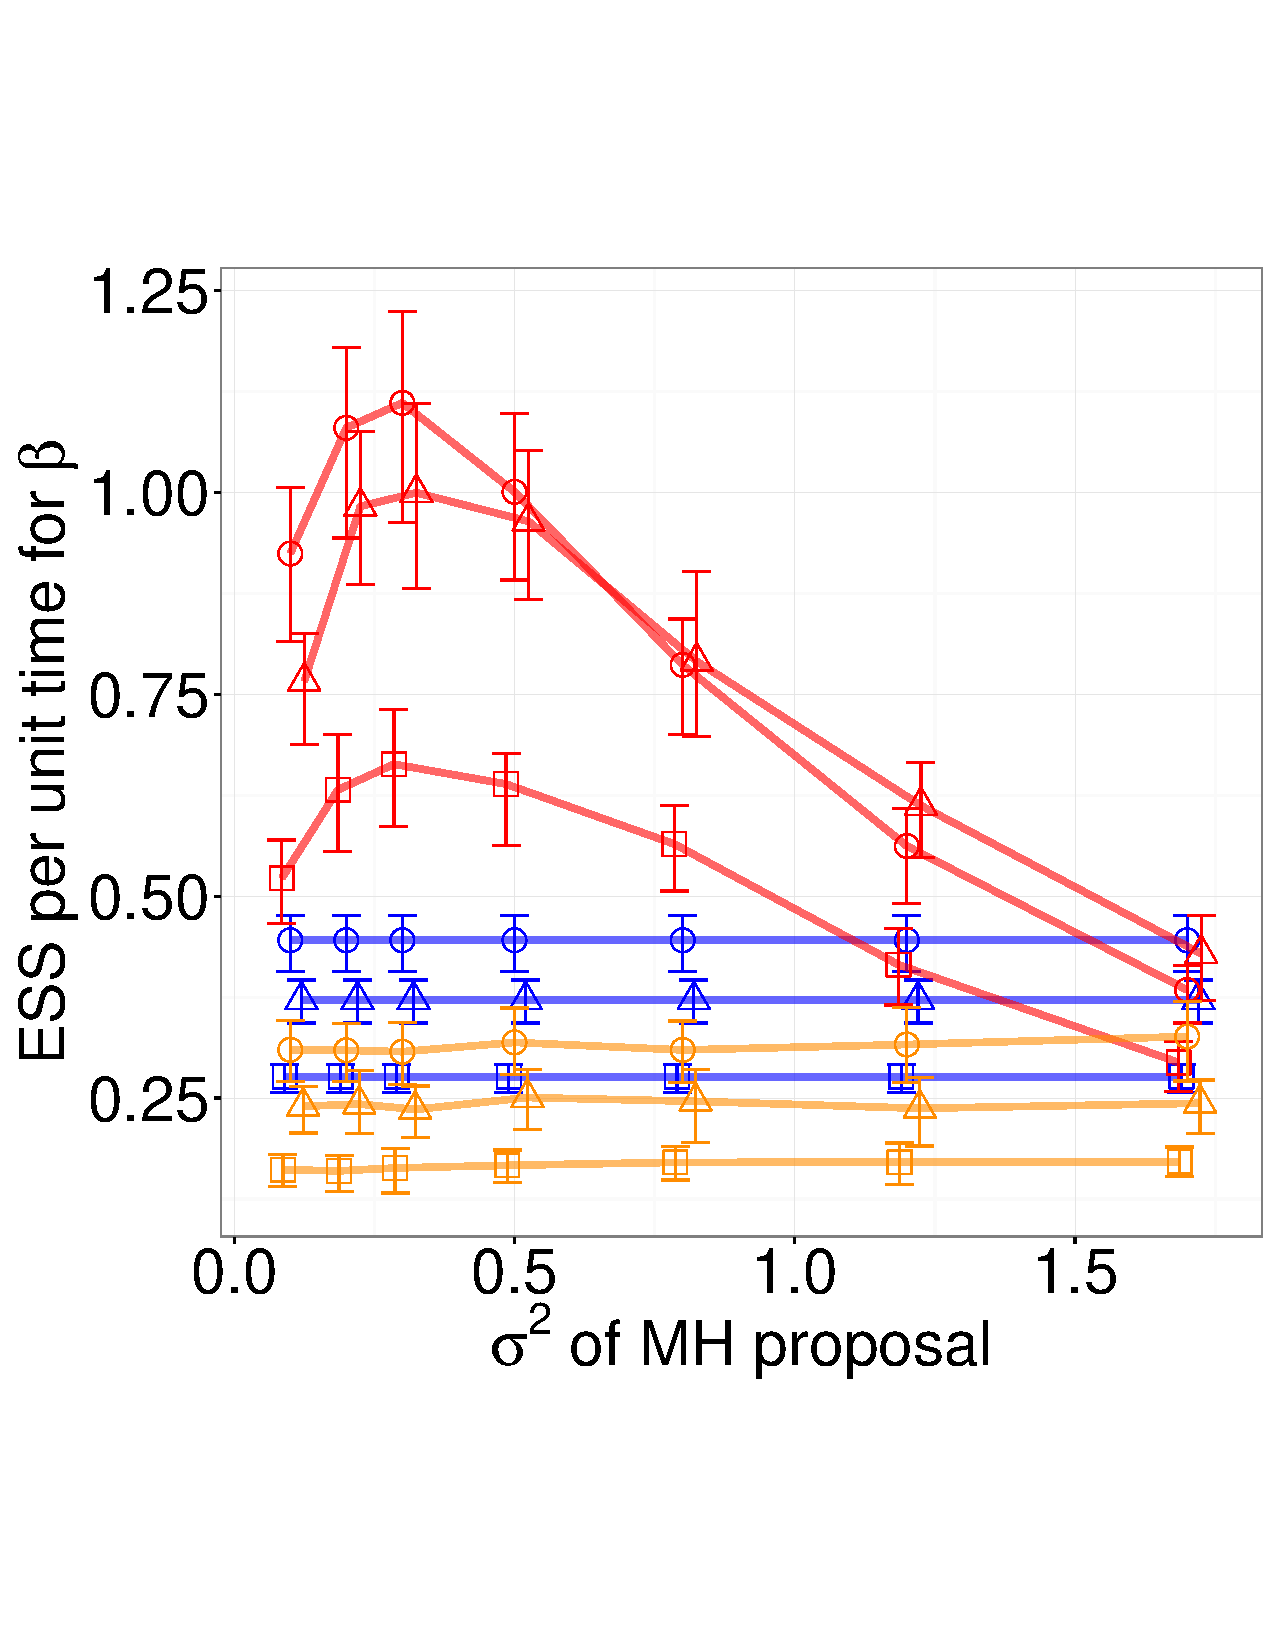
\includegraphics [width=0.950\textwidth, angle=0]{figs/pc_5_beta.pdf}
    \vspace{-0 in}
     \label{fig:ESS_pc_5}
  \end{minipage}
    \caption{ESS/sec for the nonhomogeneous immigration model (dim 5).The left is 
    for $\alpha$, and the right is for $\beta$.}
  \end{figure}

  \subsection{Immigration models with capacity}
  Below we include derivations of the posterior update rules for the immigration
  model with capacity.

  \noindent Assume our current state consists of a trajectory $S(t) \equiv (S,T)$,
  with: $S = [S_0,S_1, ...,S_n] \;, T = [t_0(t_{start}), t_1,...,t_n, t_{n+1}(t_{end})]$, and $y$ as observations.\\
Recall the definition of the immigration model. The state space is 
$\{0, 1, 2, ..., N - 1 \}$, representing the total population. The transition matrix is defined as follows. 
\begin{align*}
&-A_i =: A_{i,i} = -(\alpha + i\beta), \; \; i =0,1,...,N - 1 ;\\
&A_{i, i+1} = \alpha, \; \; i =0,1,...,N-2;\\
&A_{i, i-1}  = \beta, \; \;  i =1,...,N - 1.
\end{align*} And all the other elements are $0$.
%$$A_i =: A_{i,i} = -(\alpha + i\beta), \; \; i =0,1,...,N$$ $$A_{i, i+1} = \alpha, \; \; i =0,1,...,N-1,$$ $$A_{i, i-1}  = \beta, \; \;  i =1,...,N.$$
The conditional density(given $\alpha,\; \beta$) of a MJP trajectory $(s_0, S, T)$ in time interval $[t_{start}, t_{end}]$, with $S=(s_1, s_2,..., s_n)$, $T=(t_1, t_2,..., t_n)$ is 
$$f(s_0,S,T| \alpha, \beta) = \prod_{i=0}^{n-1} A_{s_i, s_{i+1}} \exp(\sum_{i=0}^{n} A_{s_i}(t_{i+1} - t_{i})).$$
%where $t_0 = t_{start}$, $t_{n+1} = t_{end}.$\\
%Let's denote some notations here.\\
Define
\begin{align*}
&U(s_0, S, T):= \sum_{i=0}^{n-1} \mathbb{I}_{\{s_{i+1} - s_i = 1\}} ; \\
&D(s_0, S, T):= \sum_{i=0}^{n-1} \mathbb{I}_{\{s_{i+1} - s_i = -1\}}.
\end{align*}
%$$U(s_0, S, T):= \sum_{i=0}^{k-1} \mathbb{I}_{\{s_{i+1} - s_i = 1\}}.$$
%$$D(s_0, S, T):= \sum_{i=0}^{k-1} \mathbb{I}_{\{s_{i+1} - s_i = -1\}}.$$
Let us call them U and D for short. Denote the total time when the trajectory state stays at state i as $\tau_i$, i.e. $\tau_i = \sum_{j=0}^{n} (t_{j+1} -t_j)\mathbb{I}_{\{s_j = i\}}$, then $\sum_{i=0}^n (t_{i+1} - t_i)s_i = \sum_{i=0}^{N - 1} \tau_ii.$
$$f(s_0,S,T| \alpha, \beta) = \exp(-\alpha(t_{end} - t_{start}- \tau_N) )\alpha^U \cdot  \exp((-(\sum_{i=0}^k (t_{i+1} - t_i)s_i)\beta) \prod_{i=1}^{N - 1} i^{\sum_{j=0}^{k-1}\mathbb{I}_{s_{j+1} = i -1 \;,  s_j = i} }   \beta^D$$\\
We place Gamma$(\mu, \lambda)$ and Gamma$(\omega,  \theta)$ priors on the parameters $\alpha$ and $\beta$,
%If we assume the prior of $\alpha$, and $\beta$ are $Gamma(\mu,\lambda)$, $Gamma(\omega, \theta)$, which are independent with each other. \\
%$$p(\alpha) = \frac{\lambda^\mu}{\Gamma(\mu)}\alpha^{\mu -1}e^{-\lambda \alpha}. $$
%$$p(\beta) = \frac{\theta^\omega}{\Gamma(\omega)}\beta^{\omega -1}e^{-\theta \beta}. $$
and then the posterior distribution $f(\alpha, \beta | s_0,S,T)$ is as follows:
$$ f(\alpha, \beta | s_0,S,T) \propto \exp(-(\lambda + t_{end} - t_{start}- \tau_{N - 1})\alpha) \alpha^{\mu + U -1} \cdot \exp(-(\sum_{i=0}^n (t_{i+1} - t_i)s_i + \theta)\beta) \beta^{\omega+ D -1}.$$
Thus, the posterior distributions of $\alpha$, $\beta$ are still independent. In
particular,
\begin{itemize}
\item $\alpha | s_0,S,T$ is Gamma$(\mu+ U,\lambda + t_{end} - t_{start}- \tau_{N - 1})$ distributed.\\
\item $\beta | s_0,S,T$ is Gamma$(\omega+ D,\theta + \sum_{i=0}^n (t_{i+1} - t_i)s_i)$ distributed, which is equivalent to Gamma$(\omega+ D,\theta +\sum_{i=0}^{N - 1} \tau_ii)$.\\
\end{itemize}
Such immigration models have perfectly conjugate posterior distributions when we 
assign Gamma priors to $\alpha$ and $\beta$. 
